%\documentclass[11pt,draftcls,onecolumn]{IEEEtran}
\documentclass[11pt,twocolumn,twoside]{IEEEtran}
%\documentclass[9pt,twocolumn,twoside]{IEEEtran}
\usepackage{graphicx}
\usepackage{latexsym}
\usepackage{amsmath,amssymb,amsfonts}
\usepackage{bm}
\usepackage{url}
\usepackage{balance}
\usepackage{algorithm}
\usepackage{algorithmic}
\usepackage{subfigure}
\usepackage{flushend}
\usepackage{tabularx}
\usepackage[square,numbers,sort&compress]{natbib}
\usepackage{color}
\newcommand{\MyCaption}[1]{\caption{#1}}

%\ifCLASSINFOpdf
%
%\else

\hyphenation{op-tical net-works semi-conduc-tor}

\begin{document}

\title{A Deep Look Into Educational Videos Indexing}
\author{Junjie~Cai,
        Michele Merler,~\IEEEmembership{Member,~IEEE},
        Sharath Pankanti,~\IEEEmembership{Fellow,~IEEE},
        and~Qi~Tian,~\IEEEmembership{Member,~IEEE}
\thanks{Copyright (c) 2010 IEEE. Personal use of this material is permitted.
However, permission to use this material for any other purposes must
be obtained from the IEEE by sending a request to pubs-permissions@ieee.org.}% <-this % stops a space
\thanks{J. Cai and Q. Tian are with the University of Texas at San Antonio, 78256, USA
(email: caijunjieustc@gmail.com).} % <-this % stops a space
\thanks{M. Merler and S. Pankanti is with IBM Thomas J Watson Research Center, 1101 Kitchawan Rd, Yorktown Heights, NY, 10598}% <-this % stops a space
}

\markboth{IEEE TRANSACTIONS ON MULTIMEDIA, VOL. X, NO. XX, MONTH YEAR}%
{Junjie Cai \MakeLowercase{\textit{et al.}}: A Deep Look Into Educational Videos Indexing}

\maketitle



\begin{abstract}
In the last decade, the explosive growth of online learning videos has gathered a wealth of attention from both industry and academia communities. With such a large scale of educational content on the Web, how to automatically index and organize these videos has become an interesting and challenging task.
Moreover, there exist a large quantity of educational videos containing a variety of visual content ranging from natural landscapes to classrooms, from animations to kids, from animals to plants, \emph{etc}. This constitutes of a special class of educational videos which thus far has not been investigated under the perspective of visual indexing, since all efforts on educational content indexing have been focused on more traditional lecture style videos.


Inspired by the recent progress of semantic-based approaches on indexing unconstrained consumer videos, we investigate the performance of semantic visual classifiers applied to the educational video data domain. In this paper, we propose to build a set of visual classifiers targeting at a real-world dataset of educational videos.
which contains $370$ clips of videos with more than 30 thousands key frames provided from non-lecture education collection. Moreover, to enhance the discriminative power of the proposed classifiers by complementing traditional low level descriptors, we leverage state-of-the-art deep learning features and test them in the educational video indexing domain, as opposed to the traditional one of natural images classification. Extensive retrieval experiments on two real-world datasets of educational videos using our visual content classifiers demonstrate the effectiveness of the proposed approach assisted by deep features.

%In the last decade, the explosive growth of online educational videos has gathered a wealth of attention from both industry and academia community.
%With innumerous video contents on the web, how to automatically index and organize these video has become an interesting and challenging task.
%Inspired by the recent progress of semantic-based approaches on indexing unconstrained consumer videos, we investigate the performance of semantic visual classifiers applied to the educational video data domain. In this paper, we propose to build a set of visual classifiers targeting at real-world videos.
%Moreover, to enhance the discriminative power of the proposed classifiers, we leverage state-of-the-art deep learning features and test them in the educational video indexing domain, as opposed to the traditional one of natural images classification. Extensive experiments on a real-world dataset of educational videos demonstrate the effectiveness of the proposed approach.
\end{abstract}

\begin{IEEEkeywords}
Deep Learning, Educational Video Indexing.
\end{IEEEkeywords}

%%%%%%%%% BODY TEXT

\section{Introduction}
In Web 2.0 era, online education is a popular way for students to
acquire novel knowledge in a self-paced and asynchronous way. In the last decade, the explosive growth of online learning videos has enabled people to connect, express their ideas, and share interests~\cite{survey}. Popular online
learning websites including
Coursera\footnote[1]{http://www.coursera.org},
Udacity\footnote[2]{http://www.udacity.com/},
MIT Open CourseWare\footnote[3]{http://ocw.mit.edu}and
Udemy\footnote[4]{http://www.udemy.com/}
regularly post instructors' lectures as video clips for the fruition of a wider  audience. Sites like Videolectures\footnote[5]{http://videolectures.net/} work as public venues where recorded author's academic presentation videos are shared. TED\footnote[6]{http://www.ted.org} and YouTube EDU\footnote[7]{http://www.youtube.com/edu} are popular for sharing and expressing
novel technology ideas. Youtube also features channels with education specific content such as SciShow, STEMBite and CrashCourse. Many companies run corporate training via instructional videos, and traditional publishers of educational content such as Pearson\footnote[8]{http://www.pearson.com/} are producing increasingly more video content to complement and/or substitute traditional media. Some exemplar educational videos and key frames extracted from them are illustrated in Figure \ref{fig:fig1}.

\begin{figure}
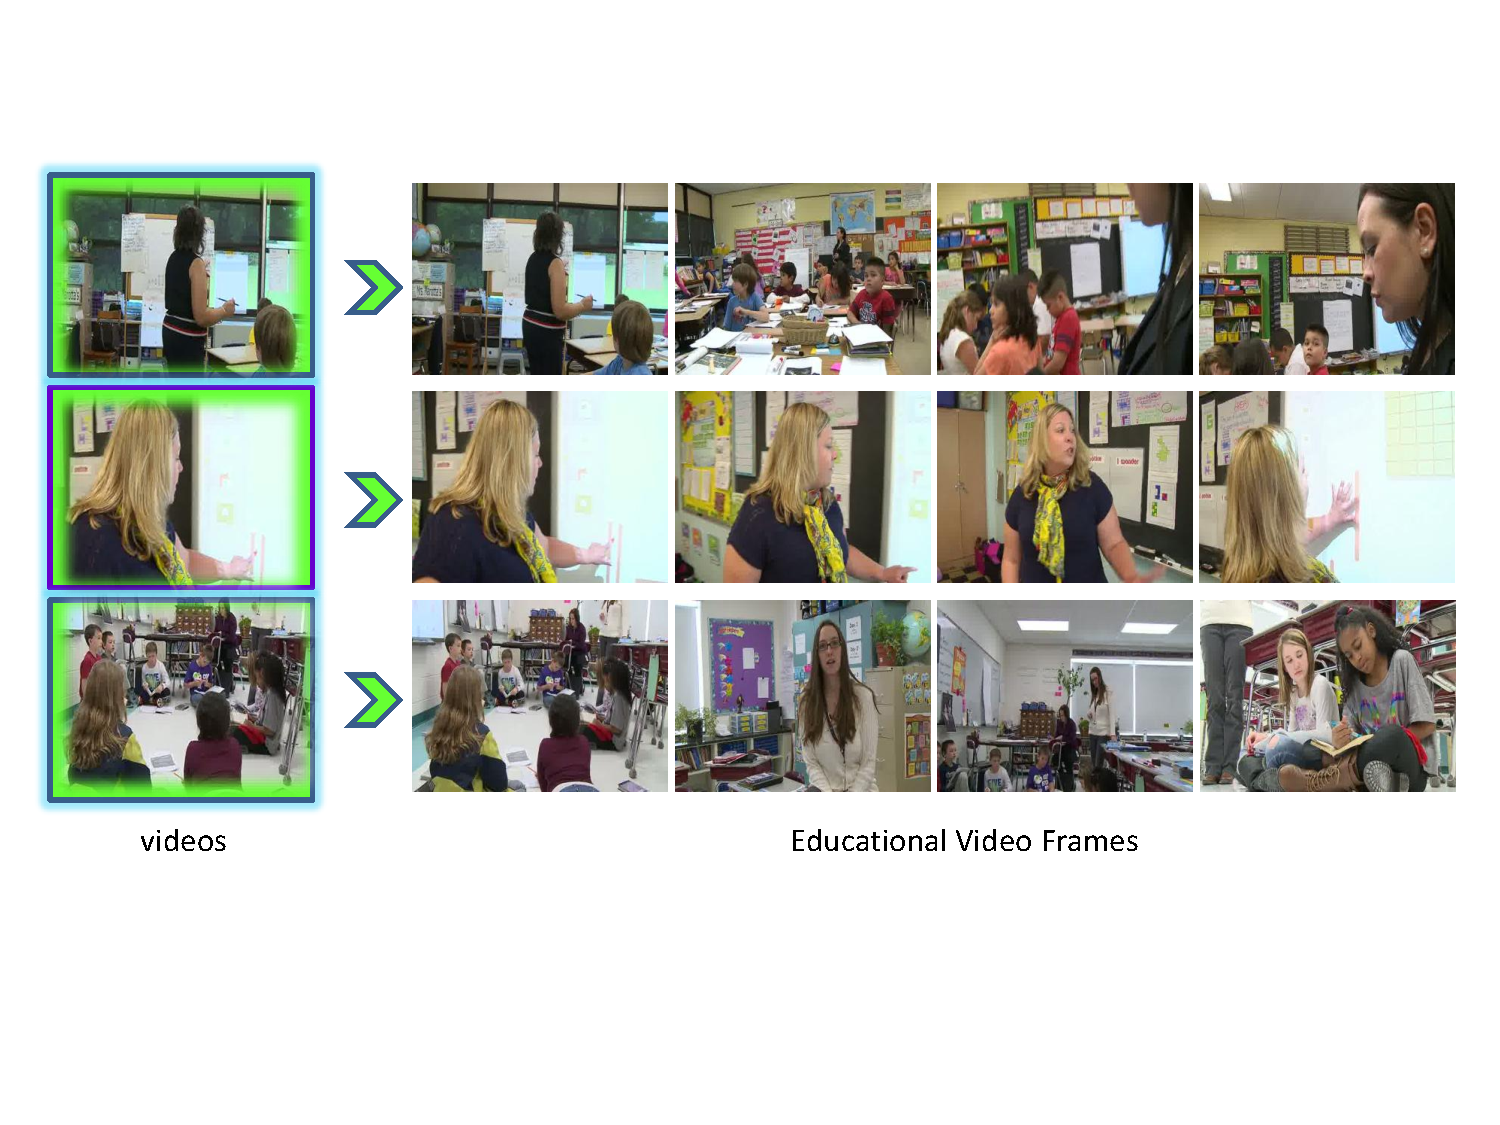
\includegraphics[width=0.48\textwidth]{fig1.pdf}
\caption{Example of educational online learning videos and extracted frames.% The original video clips are provided on \textbf{supplementary material}.
}
 \label{fig:fig1}
\end{figure}

\begin{figure*}[t]
\centering
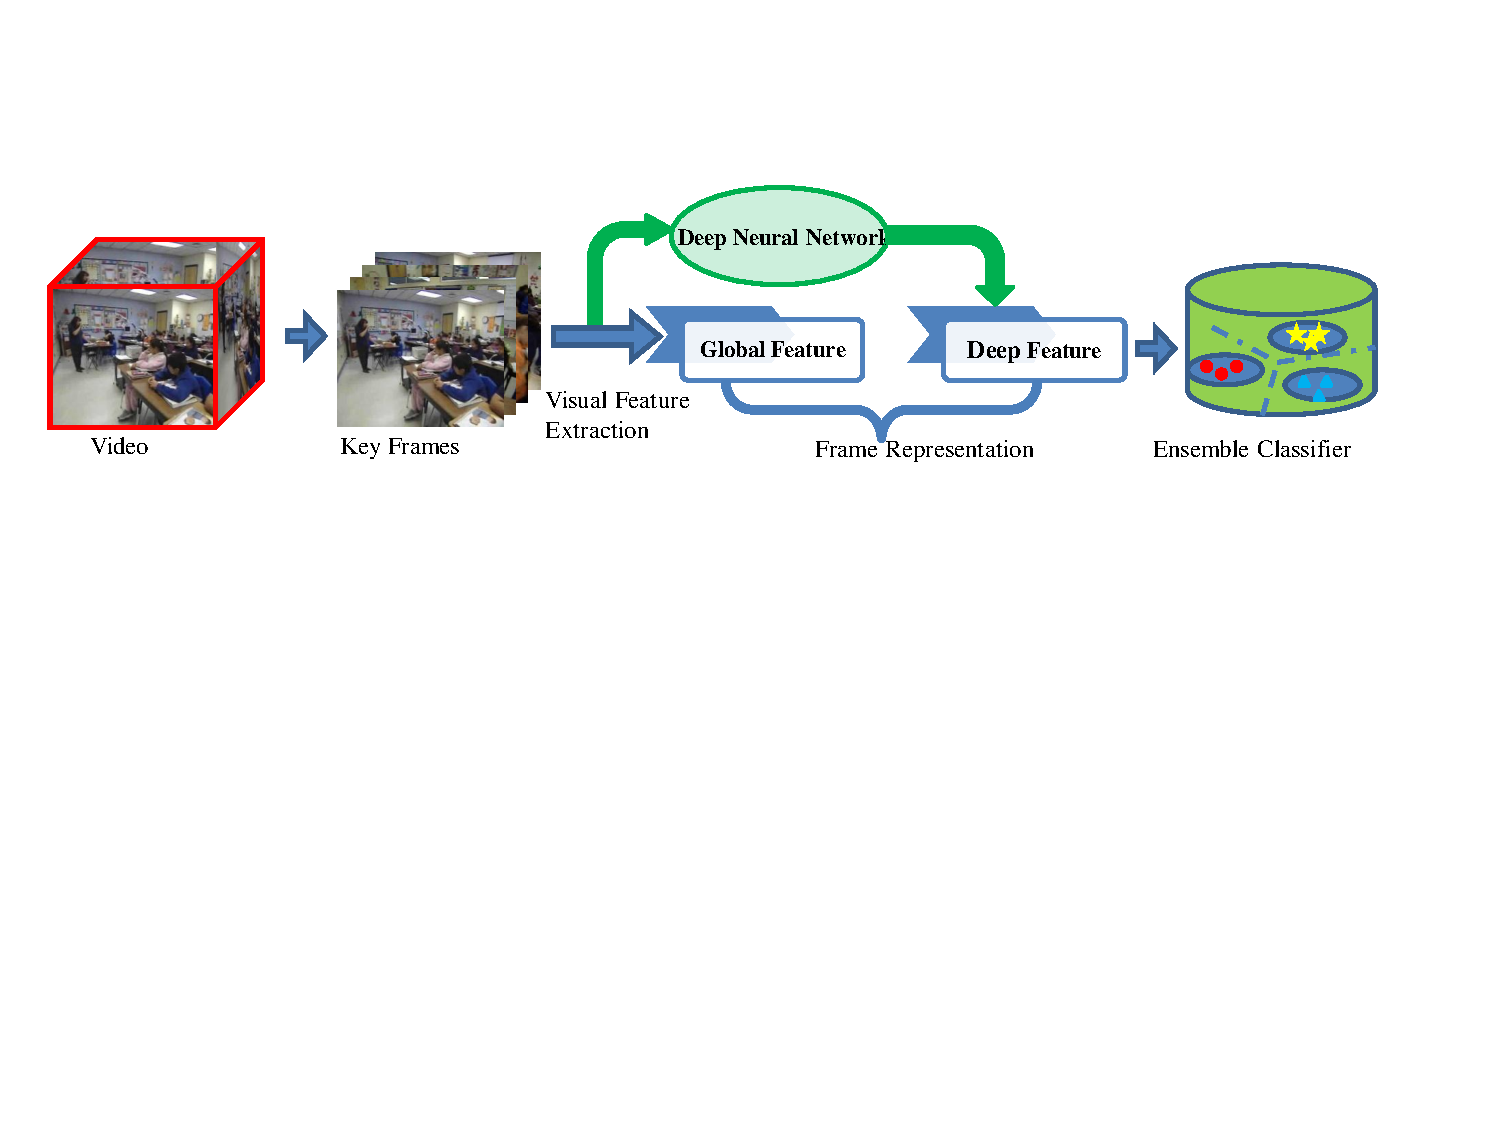
\includegraphics[width=0.9\textwidth]{fig2.pdf}
\caption{Pipeline of the proposed educational visual classifier with deep features on online educational videos. } \label{fig:fig2}
\end{figure*}


With such a great number of educational videos gathered from the Web, automatically classifying and indexing those videos is an interesting and challenging task.
To date, many state-of-the-art online learning platforms leverage
text retrieval techniques to search for relevant educational videos. Specifically, text-based approach for video classification uses the meta-data of videos such as title, speaker's profile, tagged data or abstract associated with the videos. However, when academic videos are crawled and gathered from the Web, identifying and extracting such metadata is non-trivial and erroneous task, as many of videos do not have accurate meta-data to be used.
Hence, one crucial aspect to enhance classification performance is to build visual classifiers targeted on educational video frames, which will greatly facilitate users to better index and search video content. A significant body of work has been dedicated to generate visual or multimodal indexes of university style lectures ~\cite{VastMM}\cite{talkminer}. In this context, slides and speech are dominant, and targeted slide and text detection approaches have been shown to work reasonably well. However, there exist a large quantity of educational videos (for example the aforementioned Science shows or from publishers) containing a variety of visual content ranging from natural landscapes to classrooms, from animations to kids, from animals to plants, \emph{etc}. This constitutes a special class of educational videos which thus far has not been investigated under the perspective of visual indexing, since all efforts on educational content indexing have been focused on more traditional lecture style videos.

In order to fill such gap, we propose a set of visual classifiers focusing on categories which are related to educational content, but complement existing efforts on slide detection and OCR.



Inspired by the recent progress of semantic model vector on unconstrained real-world videos~\cite{Michele_TMM13}\cite{Boostroost}, we
investigate the performance of semantic visual classifiers in our application domain containing educational video data. Different from prior work~\cite{ICME03}\cite{ICME06}\cite{IMARS}, we explore the effectiveness of deep learning features for video indexing, and employ them as a complementary cue with respect to traditional global descriptors.


In this work, we apply deep learning features obtained from the last layers of a network learned from the ImageNet dataset, to the domain of video indexing. While deep features have been successfully employed for various image classification tasks, their utilization in the video domain has been only recently introduced by Karpathy et al. \cite{Karpathy_CVPR14} in the particular domain of action classification.
 The video indexing domain we explore in this work is made additionally challenging  by need for the temporal localization, since a person performing a query is interested only in a given segment of the video, not in the whole clip, especially when the video is long. We address this issue by indexing directly keyframes instead of aggregating scores from keyframes to the entire video clip.

 We evaluate our indexing approach on a challenging real-world educational video dataset,
which contain $152,919$ Web images as training images and $30,643$ key frames extracted from nonlecture educational videos clips.   Table \ref{tab:frames} illustrated the detailed information about our dataset.
Figure \ref{fig:fig2} illustrates the flowchart of our approach. Given an educational video clip, we extract both low level global features and deep features from its key frames. We then employ a set of our pre-built classifiers to predict the concepts appearing in the key frames. The experimental results revealed that the proposed framework employing deep features is able to produce more accurate retrieved results in comparison with global features alone for this educational video search task, achieving a mean Average Precision performance of 0.42.

\begin{table}[h]\scriptsize
  \centering
  \caption{Number of Keyframes from our real-world Scalable Dataset. }
    \begin{tabular}{|l|c|c|c|}

    \hline
    NON-LECTURES & Keyframes & Avg Keyframes/video & Videos \\
    \hline
    \hline
    STEMbite & 1472  & 24    & 61 \\
    Scishow  & 10482 & 23    & 450 \\
    Crashcourse & 17676 & 80    & 221 \\
    Pearson & 867   & 16    & 54 \\
    NICA  & 5415  & 57    & 95 \\
    \hline
    \hline
    TOTAL & 35912 & 40    & 370 \\
    \hline
    \end{tabular}%
  \label{tab:frames}%
\end{table}%

The main contributions of this paper are the followings:
\begin{itemize}
    \item We explore the state-of-the-art deep learning feature extracted with both ImageNet model and self-trained CNN model. We investigate its performance in comparison with conventional global features.
    \item We contribute a real-world educational video datasets, including one toy dataset and one scalable dataset. The scalable dataset contain $152,919$ Web images as training images and $30,643$ key frames extracted from nonlecture educational videos clips.
    \item Targeting on the domain of online educational videos, we conduct extensive experiments with the proposed educational classifier and demonstrate its effectiveness assisted with deep features.
\end{itemize}

The rest of this paper is organized as follows. Firstly, we provide a review of the related work on video recognition and indexing in Section II. The proposed education visual classifier framework is elaborated in Section III.
Specifically, we elaborate global features, low-level features and deep features from Section \ref{subsec1} to Section \ref{subsec3}, respectively. The proposed educational visual classifiers is detailed in Section \ref{subsec4}.
In Section IV, we report our experimental results on a real-world educational video dataset, followed by the conclusions in Section V.

\section{Related Work}
In this section, we provide a briefly description of the existing video indexing approaches, review the deep learning features exploited in recent literature, and describe their application on video domain.
\subsection{Video Indexing}

Video recognition research has been largely driven by the advances in image recognition methods, which were often adapted and extended to
deal with video data. A large family of video action recognition methods is based on shallow high-dimensional encodings of local
spatio-temporal features. For instance, the algorithm of \cite{Laptev_CVPR08} consists in detecting sparse spatio-temporal interest points, which
are often described using local spatio-temporal features: Histogram of Oriented Gradients~(HOG)~\cite{HOG} and Histogram of Optical Flow~\cite{HOF}.
The features are then encoded into the Bag-of-Features (BoF) representation, which is pooled over several spatio-temporal grids (similarly to spatial
pyramid pooling) and combined with an SVM classifier. In a later work \cite{WangHeng_BMVC09}, it was shown that dense sampling of local features outperforms
sparse interest points.

Instead of computing local video features over spatio-temporal cuboids, state-of-the-art shallow video representation \cite{WangHeng_ICCV13} make use of dense
point trajectories. The approach, first introduced in \cite{WangHeng_CVPR11}, consists in adjusting local descriptor support regions, so that they follow dense
trajectories, computed using optical flow. The best performance in the trajectory-based pipeline was achieved by the Motion Boundary Histogram (MBH)~\cite{HOF}, which is
a gradient-based feature, separately computed on the horizontal and vertical components of optical flow. A combination of several features was shown to further boost
the accuracy. Recent improvements of trajectory-based shallow representation include compensation of global (camera) motion \cite{Jegou13} and the use of
the Fisher vector encoding~\cite{fishervector} for trajectory features~\cite{WangHeng_ICCV13}.

\subsection{Deep Learning Features}
Deep learning features have been shown to set the state-of-the-art in many applications such as
OCR~\cite{YLecun}, speech recognition~\cite{SpeechRecogntion} and object detection~\cite{ImageNet_challenge}.
Researchers have also developed a myriad of approaches as well as toolkits with deep learning features to tackle the challenging problems in various research areas.
For instance, Attila~\cite{Attila} and Kaldi~\cite{Kaldi} for speech recognition, Overfeat~\cite{OverFeat}, CAFFE~\cite{CAFFE} and Cuda-convnet~\cite{Alex_NIPS12} for visual applications, Theano~\cite{Theano} for natural language processing or more general learning purpose.


There has also a number of attempts to develop a deep architecture for video recognition. In the majority of these works, the input to the network is a stack of consecutive video
frames, so the model is expected to implicitly learn correspondences or spatio-temporal motion-dependent features in the first layers, which can be a difficult task.
In \cite{huang07}, an HMAX architecture for video recognition was proposed with pre-defined spatio-temporal filters in the first layer. Later, it was combined~\cite{HMDB}with a
spatial HMAX model, thus forming spatial (ventral-like) and temporal (dorsal-like) recognition streams. Unlike our work, however, the streams were implemented as hand-crafted and rather shallow (3-layer) HMAX models. In \cite{Fergus10}, a convolutional RBM was used for unsupervised learning of spatio-temporal features, which were then plugged into a ConvNet for action classification. Discriminative end-to-end learning of video ConvNets has been addressed in \cite{Kaiyu13} and, more recently, in~\cite{CVPR14}, who compared several
ConvNet architectures for action recognition. Training awas carried out on a very large Sports-1M dataset, comprising 1.1M Youtube videos of sports activities. Interesting, \cite{CVPR14} found that a network, operating on individual video frames, performs similarly to the networks, whose input is a stack of frames. This might indicate that the learnt spatio-temporal features do not capture the motion well. The learnt representation, fine-tuned on the UCF-101 dataset, tuned out to be 20\% less accurate than hand-crafted stat-of-the-art trajectory-based representation~\cite{Early_Fusion}.

\section{Educational Visual Classifiers}
In this section, we illustrate our approach for extracting global features, low-level features and deep features. Then we provide a formal description of the proposed educational visual classifiers on top of them.

\subsection{Global Features}\label{subsec1}

We extract three types of global visual descriptors including color, texture and edges to represent each image. %The feature list are denoted in Table \ref{tb:feat}.
\begin{itemize}

\item \textbf{COLOR}: Color descriptors consist of color correlogram, color histogram and color wavelet features. In HSV color space, Color correlogram is a global color and structure feature
which can be represented by 166-dimensional single-banded auto-correlogram using 8 radii depths. Color histogram is a 166-dimensional histogram feature vector in the same HSV space. Color moments are extracted from a 5*5 grid and represented by the first 3 moments for each grid region in Lab color space as a normalized 255-dimensional vector.

\item \textbf{TEXTURE}: Texture descriptor contains wavelet texture, GIST and LBP histogram features.  Wavelet texture is localized texture extracted from a 3*3 grid and represented by the normalized 108-dimensional vector of the variances in 12 Haar wavelet sub-bands for each grid region.  To compute the GIST descriptor, the image is segmented by a 4 by 4 grid for which 8 orientation histograms of 4 scales are extracted and produces a 512-dimensional feature vector. The LBP histogram feature contains 58 uniform and 1 non-uniform pattern.

\item \textbf{EDGE}: the Edge histogram feature is computed with 8 edge direction bins and 8 edge magnitude bins which is based on a Sobel filter,  resulting in a 64-dimensional feature vector.

\end{itemize}

We observe that having a large diversity of visual descriptors is important for capturing different semantics and dynamics in the video scene, as reported in previous works ~\cite{Michele_TMM13}.
Moreover, we extract the descriptors at different spatial granularities ~(i.e., global, layout, pyramid, horizontal parts, grid, horizontal center, vertical center). Such spatial divisions have shown improved performance and robustness in video retrieval benchmarks~\cite{TRECVID07}. In sum, we extracted 47 different kinds of features for the classifiers training.

\subsection{Low-level Features with Fisher Vector Representation}\label{subsec2}

Fisher Vector (FV) coding approach, derived from Fisher Kernel, was originally proposed for large scale image classification.
Compared with other coding methods such as vector quantization and sparse coding, FV coding can easily obtain high-dimensional feature codes with
small codebook size, which has been shown to provide considerable performance improvements when utilizing linear classifiers.

Following best practices reported in the literature~\cite{Early_Fusion}, we process the descriptors independently.
We extract SIFT low-level visual features and leverage the GMM model followed by Fisher Vector over the features extracted from all the Web images.
Specifically, we first densely extract local SIFT descriptors with a spatial stride of 4 pixels at 9 scales and the width of SIFT spatial bins is fixed as 8 pixels, which
are the default settings in the VLFeat toolbox~\cite{VLFeat}. We learn a GMM dictionary sampled from a subset of one million SIFT descriptors. All descriptors are
whitened after PCA processing to 64-dimension with a ratio of 0.5. We then conduct FV encoding and apply $\ell_{2}$ normalization to the resulting super vectors.



\subsection{Deep Features}\label{subsec3}

\subsubsection{ImageNet Model}
Inspired by the success of deep learning framework on large-scale visual recognition tasks such as classification,
embedding and object detection~\cite{ImageNet_challenge}, we first employ it as the feature extractor for video frames. For the implementation, we utilize the open
source deep learning framework CAFFE~\cite{CAFFE}, which is based on the deep convolutional neural network architecture by
Krizhevsky et al. \cite{Alex_NIPS12}. In fact, our testing query and database frames are independent from the ImageNet dataset,
hence we use the pre-trained ImageNet model for ILSVRC image classification from \cite{LSVRC}, as an analog to using the prior knowledge
a human obtained from previous visual experiences to learn new tasks more efficiently.

The activations of the neurons in the late hidden layers could be used as strong features for a variety of video recognition tasks because
they contain much richer semantic representations than any earlier convolutional layer in the network. Therefore, we use features from the last
three layers in our implementation, which are the first set of activations that have been fully propagated through the convolutional layers
of the network, the final hidden layer~(i.e.,~just before propagation through the final fully connected layer to produce the class predications) and
the layer between them. We set the network input with mean-centered raw RGB pixel 256 $\times$ 256 images, the values are forward propagated through 5
convolutional layers~(i.e., pooling and ReLU non-linearities) and 3 fully-connected layers (i.e., to determine its final neuron activities), finally we obtain the 4096-dimension vector for the last hidden layers and normalize the vectors by their $\ell_{2}$ normalization.
\subsubsection{Our CNN Model}

We train our own model to obtain the deep feature representation based on the Convolutional Neural Network (CNN). The convolutional network consists of several layers and each
layer is a linear transformation followed by a non-linear one. The first layers takes an 227 $\times$ 227 $\times$ 3 input image as the input. The network is based on
the architecture used in \cite{CAFFE}. Each layer consists of: (1) convolutional of the previous layer output with a set of filters; (2) passing the responses through
a rectified linear function. To obtain the CNN model, we divide our dataset (including $152,919$ images) into two parts,the training part contains 80\% of Web images and validation dataset with the rest of 20\% images.
We describe the  in


\begin{table}[h]
 \centering \caption{Global visual features extracted for visual classifiers.}
\begin{tabular}{|c|c|c|}
\hline  Color  &  Texture   & Edge   \\
\hline
\hline color correlogram &lbp histogram    & edge histogram       \\
\hline  color histogram  &GIST    & -   \\
\hline  color wavelet    &wavelet texture & - \\
\hline
\end{tabular}
\label{tb:feat}
\end{table}



\begin{table}[h]\scriptsize
 \centering \caption{Notations and descriptions. }
\begin{tabular}{|l|c|}
\hline Notations        & Descriptions      \\
\hline
\hline $m$              & chi square, histogram intersection, linear approximate    \\
\hline $S_{b}$          & maximum num of positive samples per unit model            \\
\hline $N_{b}$          & maximum num of bags to try for each descriptor           \\
\hline $r_{d}$          & fraction for unit model training           \\
\hline $w$              & sum or weighted sum          \\
\hline $N_{p}$          & num of parameters to search for modeling         \\
\hline
\end{tabular}
\label{tb:para}
\end{table}
\subsection{Educational visual model learning}\label{subsec4}
For each feature type, we learn classifier models from a number of $N_{b}$ of bags of training data, randomly
sampled with a majority of positive and negative samples, with sample ratio $r_{d}$.  Specifically, one-versus-all SVMs with various kernels (Chi-square, Histogram Intersection, Linear Approximate Kernel) are trained, independently for each concept, based on each descriptor. During training for one category, all the samples from the
other categories are used as the negative examples. The default parameters for
$N_{b}$ and $r_{d}$ used to train all the base models for the semantic models are 3 and 0.3, respectively, which result in
a pool of $N = 141$ base models for each concept. To minimize the sensitivity of the parameters for each base model, we choose the SVM
parameters based on a grid search strategy. Then we build the SVM models with different values on the kernel parameters $C$, the relative
cost factors of positive versus negative samples, the feature normalization schemes, and the weights between training error and margin.
Each model is then associated with its cross validation performance, where average precision is employed as the performance measure.
Moreover, the fusion strategies of the base models into an ensemble classifier are determined based on average precision performance on the held-out data.
To reduce the risk of overfitting, we control the strength and correlation of the selected base models by employing
a greedy model selection step. The algorithm iteratively selects the most effective base model from the unit models pool, adds it to
the composite classifier without replacement, and evaluates its average precision on the held-out set.
Once the best parameters are determined, the SVMs are retrained on the whole development set. The semantic model output is
then the ensemble classifier with the highest average precision observed on the held-out set. For clarity, we illustrate several important notations and their definitions throughout the experiments in Table \ref{tb:para}.

%\begin{table}\footnotesize
% \centering \caption{Notations and descriptions. }
%\begin{tabular}{|l|c|c|}
%\hline Notations    & Variable    & Descriptions      \\
%\hline
%\hline $m$          & model string & Chi square histogram intersection linear approximate          \\
%\hline $S_{b}$          & Bag size    & Max num of pos\/neg samples per unit model            \\
%\hline $N_{b}$          & max number bags     & maximum num of bags to try for each descriptor           \\
%\hline $r_{d}$        & train fraction     & fraction for unit model training           \\
%\hline $w$       & Fusion method     & sum weighted sum          \\
%\hline $N_{p}$          & learning para     & Num para to search for modeling         \\
%\hline
%\end{tabular}
%\label{tb:dataset}
%\end{table}

\section{Experiments}
To enhance the educational classifier performance, we first conduct extensive experimental comparisons tuned with sets of various parameters. Then, we investigate deep feature performance in comparison with conventional global features.

The experiments are performed in two datasets: a toy datset and a real-world scalable dataset. The toy dataset is mainly designed for parameter tuning while the other dataset is utilized the demonstrate the
effectiveness of the proposed educational classifiers.

We implement the experiments on a server
with a $8$-core, $2.4$GHz and $24$ GB memory. We adopt Average Precision, a common choice for evaluating
visual search engines~\cite{TRECVID07}\cite{Michele_TMM13},
\begin{equation}
{\rm{AP}} = \frac{1}{{TP}}\sum\nolimits_{d = 1}^N {\frac{{T{P_d}}}{d}} {I_d}
\end{equation}
where $I_{d} = 1$ if the $d^{th}$ sample is relevant and $0$ otherwise. $TP$ is the total number of relevant samples in the collection and $N$ is the number of total samples. $TP_{d}$ denotes the number of relevant samples
found in the top $d$ ranked samples returned by the system. In addition to Average Precision, we also report overall performance of mean Average Precision~(mAP) which is averaged over the concepts.

\begin{figure}
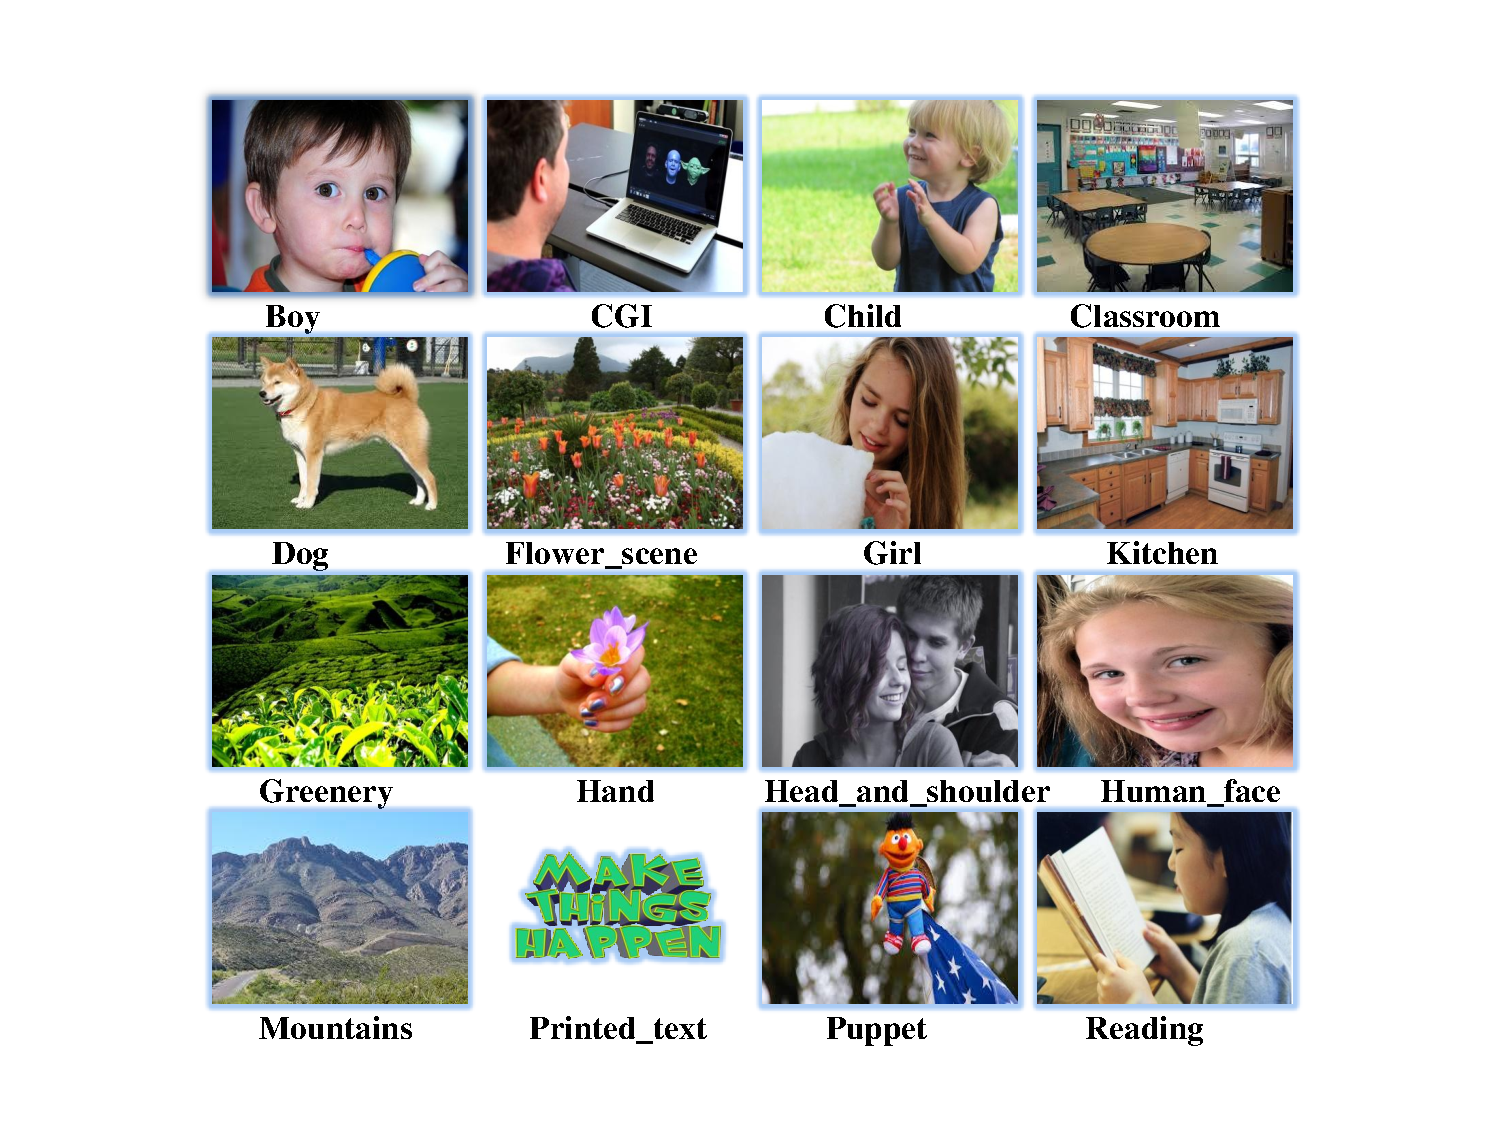
\includegraphics[width=0.48\textwidth]{fig4.pdf}
\centering
\caption{Sample images from the training dataset.} \label{fig:fig4}
\end{figure}


\begin{figure*}[t]
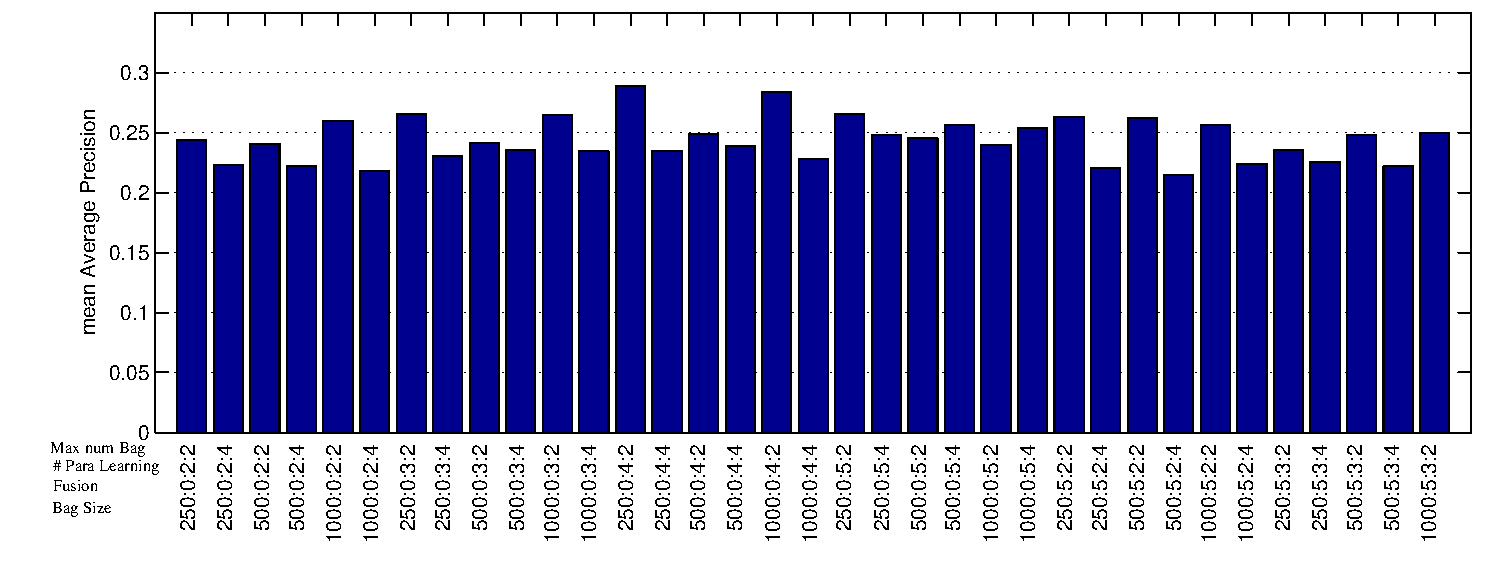
\includegraphics[width=0.85\textwidth]{fig3.pdf}
\centering
\caption{Retrieval performance comparison in mAP with global features in out dataset. The results are tuned with variables (a) max number of bags (b) number of parameter learning (c) fusion approach(sum or weighted sum) (d) bag size.} \label{fig:retrieval}
\end{figure*}

\subsection{Data and Methodologies}
\textbf{Pearson Toy Dataset:} We first collect 22,037 Web images from 16 popular concepts via public api as the toy training dataset:
``Boy", ``CGI", ``Child", ``Classroom", ``Dog",  ``Flower scene",  ``Girl", ``Greenery", ``Hands", ``Head and shoulders", ``Human face", ``Kitchen", ``Mountains", ``Printed text", ``Puppet", ``Reading''.
The test dataset contains $54$ clips of videos with average 120 seconds duration provided from Pearson education collection. We extract and select 1005 key frames from these video clips. For each frame, its relevance to the corresponding query is labeled with two levels: relevant and irrelevant which indicated by scores 1 and 0, respectively. The ground truth of each frame is manually labeled by professional image researchers. Some exemplar images of each concept are illustrated in Figure \ref{fig:fig4} and number of images and extracted video frames in training and test dataset are detailed in Table \ref{tb:dataset}.

\textbf{Scalable Dataset:} In order to further validate the proposed educational classifiers, we extend the toy dataset in a large-scale manner.  The scalable dataset contains $152,919$ Web images.
 We crawled and organized the training dataset in a hierarchical structure which contains 6 main classes and 162 subcategories. The main classes include ``Animals",``People", ``objects",``Setting",
 ``Graphical Element" and ``Activities". Table \ref{tbl:large} illustrated the detailed information about the dataset.
 The keyframes in the test dataset includes $35,912$ samples from $370$ video clips.

\subsection{Performance Evaluation in Pearson Toy Dataset}

We perform experimental evaluation with one-versus-all classifiers using global features.
During training for one concept, all the images from the other concept are used as negative examples.
In order to optimize the sensitivity of the parameters for each base model, we select parameter C from \{0.1,1,10,100\} via grid search on a 5-fold cross validation, with a 70\% training and 30$\%$ validation random splits on both
positive and negative examples of datasets.
To evaluate the retrieval performance, we empirically choose and tune four sets of important variables consisting of max number of bags, number of parameter to search for modeling, fusion method and bag size.
Figure \ref{fig:retrieval} provides the detailed performance comparison with various parameter combinations in terms of mAP.
It obtains 0.289 in mAP score when we use 250 samples per bag and 2 bags per unit model in the training set.
We observe that it achieves better performance when we set bag size as two in comparison with four bags.
This is because the over-fitting problem might occur in the experiment if we adopt higher number bags per feature.

Also, we conduct an experimental comparison between classifier with linear approximate kernel \cite{MED} and non-linear kernel~(Chi-square, Histogram-intersection).
When fixing the other parameters, we observe that the mAP of linear approximate kernel achieves 0.23 while non-linear kernel yields an mAP of 0.28.
Hence, non-linear kernel performs favorably and better than linear approximate kernel in this search task.


\begin{table}[t]\scriptsize
 \centering \caption{Number of images and extracted video frames in Pearson dataset. }
\begin{tabular}{|l|c|c|l|c|c|}
\hline Concepts     & Training      & Test   & Concepts     & Training      & Test       \\
\hline
\hline Boy          & 544           & 101    & Greenery     &  1068         & 15                 \\
\hline Reading      & 1217          &145   & Classroom    & 804           & 31              \\
\hline CGI          & 438           & 99     & Head\&Shoulders & 1625    & 340  \\
\hline Child        & 647           & 191    & Human face & 4906            & 220 \\
\hline Puppet       & 214           &128     & Kitchen      & 564           &10 \\
\hline Dog          & 2352          & 14     & Mountains    & 843           &10\\
\hline  Hands        & 1200          & 73     &Flower scene & 825           &10  \\
\hline Girl         & 710           & 86       &Printed text      & 4080          &342   \\

\hline
\end{tabular}
\label{tb:dataset}
\end{table}




\begin{table}[h]
 \centering \caption{Performance comparison between deep features and global features in mAP.}
\begin{tabular}{|c||c|c|}
\hline Feature Type      & mAP  & improvement     \\
\hline \cite{MED}        & 0.23 & -\\
\hline Global Feature    &0.28  & +21.7\%   \\
\hline Deep Feature     &\textbf{0.42}  & +82.0\%   \\
\hline
\end{tabular}
\label{tb:comp_feat}
\end{table}

%\begin{table}[h]
% \centering \caption{Experimental performance of deep learning feature on Caltech256 .}
%\begin{tabular}{|c|c|c|c|}
%\hline  Training         &  5     & 10     & 20     \\
%\hline
%\hline \cite{Classemes}  & 28.0\% & 35.2\% & 41.1\% \\
%\hline Our Feature       & 56.1\% & 63.1\% & 68.3\% \\
%\hline
%\hline Training          &30      &40      &50     \\
%\hline \cite{Classemes}  &44.9\%  &46.1\%  &49.2\% \\
%\hline  Our Feature      &70.8\%  &71.9\%  &73.0\% \\
%\hline
%\end{tabular}
%\label{tb:caltech}
%\end{table}
%
%To validate the effectiveness of the pre-trained ImageNet model, we follow the procedure in \cite{Caltech256} to evaluate it on Caltech-256 dataset that contains $30,607$ Web images. Specifically, we employ the standard approach of learning the classifier for different number of training images per class \{5, 10, 20,$\dots$, 50\}. As denoted in Table \ref{tb:caltech}, we achieve about 73.0\% for 50 training images with the pre-trained model.  The experimental result is comparable to the state-of-the-art performance reported in \cite{Fergus_ECCV14} and significantly improve the recent released result in \cite{Classemes}. Hence, we employ this pre-trained model to extract deep features for the key frames in this work.
%\begin{figure}[h]
%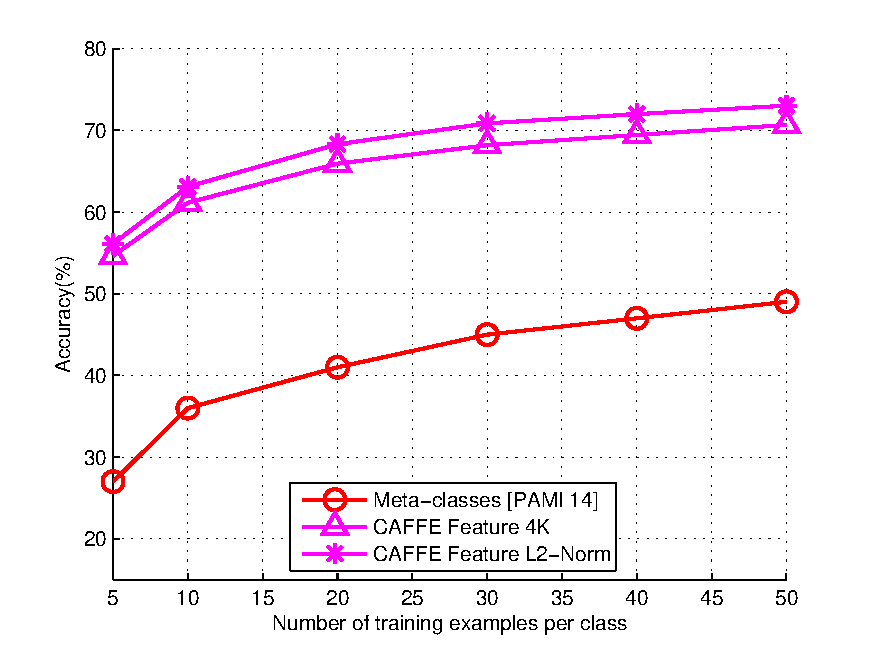
\includegraphics[width=0.5\textwidth]{fig7.pdf}
%\centering
%\caption{Detailed performance comparison on Caltech256.} \label{fig:fig7}
%\end{figure}


To enhance retrieval performance of educational classifier, we conduct the experimental comparison with deep learning features.
We use the same parameter setting as selected in the previous subsection.
The mean Average Precision overall all the concepts based on our algorithm
is also shown in Table \ref{tb:comp_feat}. Obviously from the observation above, our method with deep features achieves a mAP of
$0.42$ and obtains a noticeable improvement compared with global features.
The performance gives credits to the deep features by enhancing the discriminative power of educational classifier. Hence,
assisted with deep learning features, the experimental result demonstrates superiority of our approach over conventional global features.
Nevertheless, we notice that our algorithm is less effective
in the concepts ``Puppet" and ``Human face". And
this may result from that they share a couple of images which belong to both two categories.
%\begin{table}[h]
% \centering \caption{Performance comparison between our educational ensemble classifier and LibLinear classifier.}
%\begin{tabular}{|c||c|c|}
%\hline Approach    & mAP  &  improvement        \\
%\hline Liblinear\cite{Liblinear}    & 0.21   & -    \\
%\hline Educational Ensemble Classifier   & 0.42   & +0.21   \\
%\hline
%\end{tabular}
%\label{tb:classifier_comp}
%\end{table}

To further test the effectiveness of our proposed approach, we validate our performance in comparison with the LibLinear classifier \cite{Liblinear}
with deep features. Figure \ref{fig:fig6} provides the experimental comparison in Average Precision among all concepts and presents the score comparison in terms of mAP. It can be observed that our approach achieved significant improvement when mAP score increased from $0.21$ to $0.42$.
The above results demonstrate that the proposed approach with deep feature is more suitable in the task of educational video search.
%
%\begin{figure}[h]
%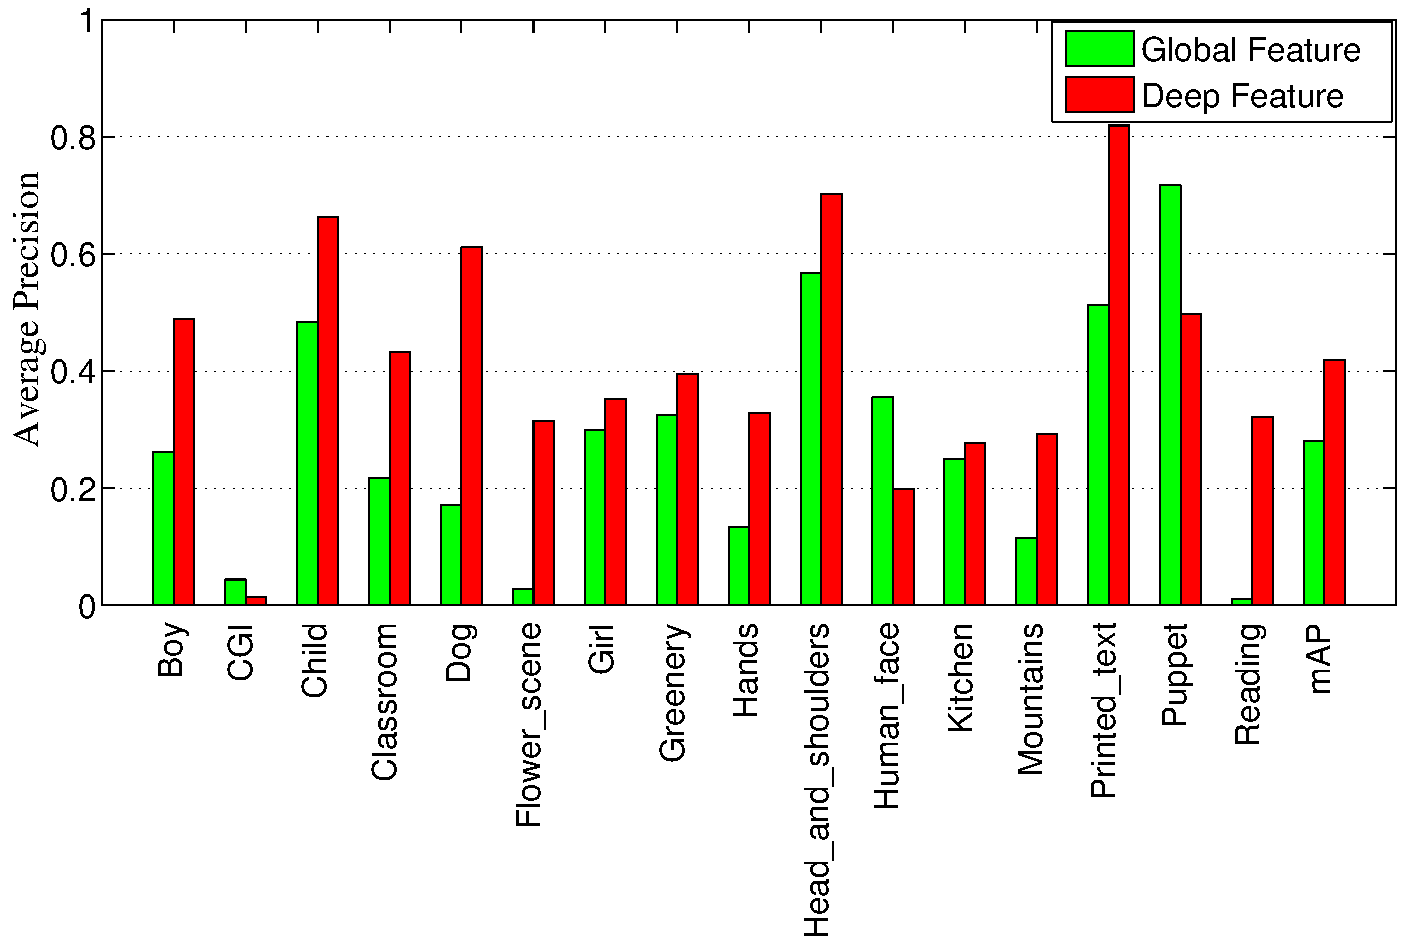
\includegraphics[width=0.48\textwidth]{fig5.pdf}
%\centering
%\caption{Detailed performance comparison over all the concepts on our dataset.} \label{fig:fig5}
%\end{figure}


\subsection{Large-Scale Evaluation with Self-Trained Model}
In order to train the deep model, we divide the scalable dataset into two parts. Specifically, the training part contains 80\% of Web images and validation dataset with the rest of 20\% images.
We implement the network under the caffe framework \cite{CAFFE} and train them using stochastic gradient descent with a batch size of 256 examples, momentum of 0.9, and
a weight decay of 0.0005. We use an equal learning rate for all layers and adjust it every 10,000 iterations. The strategy is to divide the learning rate by 10 when the validation error rate
stops decreasing with the current learning rate. The learning rate is initialized to 0.01 for the network. We set the maximus iterations as 50,000.
We train the networks for roughly 65 epochs, which takes 28 hours on one NVIDIA K40c GPU. It can rapidly process one 227 * 227 image within about 0.5 second.
% Table generated by Excel2LaTeX from sheet 'Data'

\begin{table}\scriptsize
\centering
\begin{tabular}{|l||c|}
\hline
Feature              & mAP    \\
\hline\hline
SIFT+FV                 & 53.16\%   \\
\hline
GLOBAL FEATURES                   & 33.97\%   \\
\hline
Deep Feature with Pre-trained Model &  61.55\%  \\
\hline
\hline
Self-trained Deep Model   &  61.55\% \\
\hline
\end{tabular}
\caption{Performance comparison of heterogeneous features on educational video indexing. }
\label{tb:combination}
\end{table}




\section{Conclusion}
In this paper, we investigated the state-of-the-art deep learning feature and evaluated its performance compared with conventional global features in the domain of educational video content retrieval.
We introduced an educational video retrieval system based visual classifiers
assisted with deep features, and evaluated it by conducting retrieval experiments on a real-world dataset of online learning videos.
The extensive experiments demonstrated the effectiveness of our
proposed framework in this educational video retrieval task.

\begin{figure}[h]
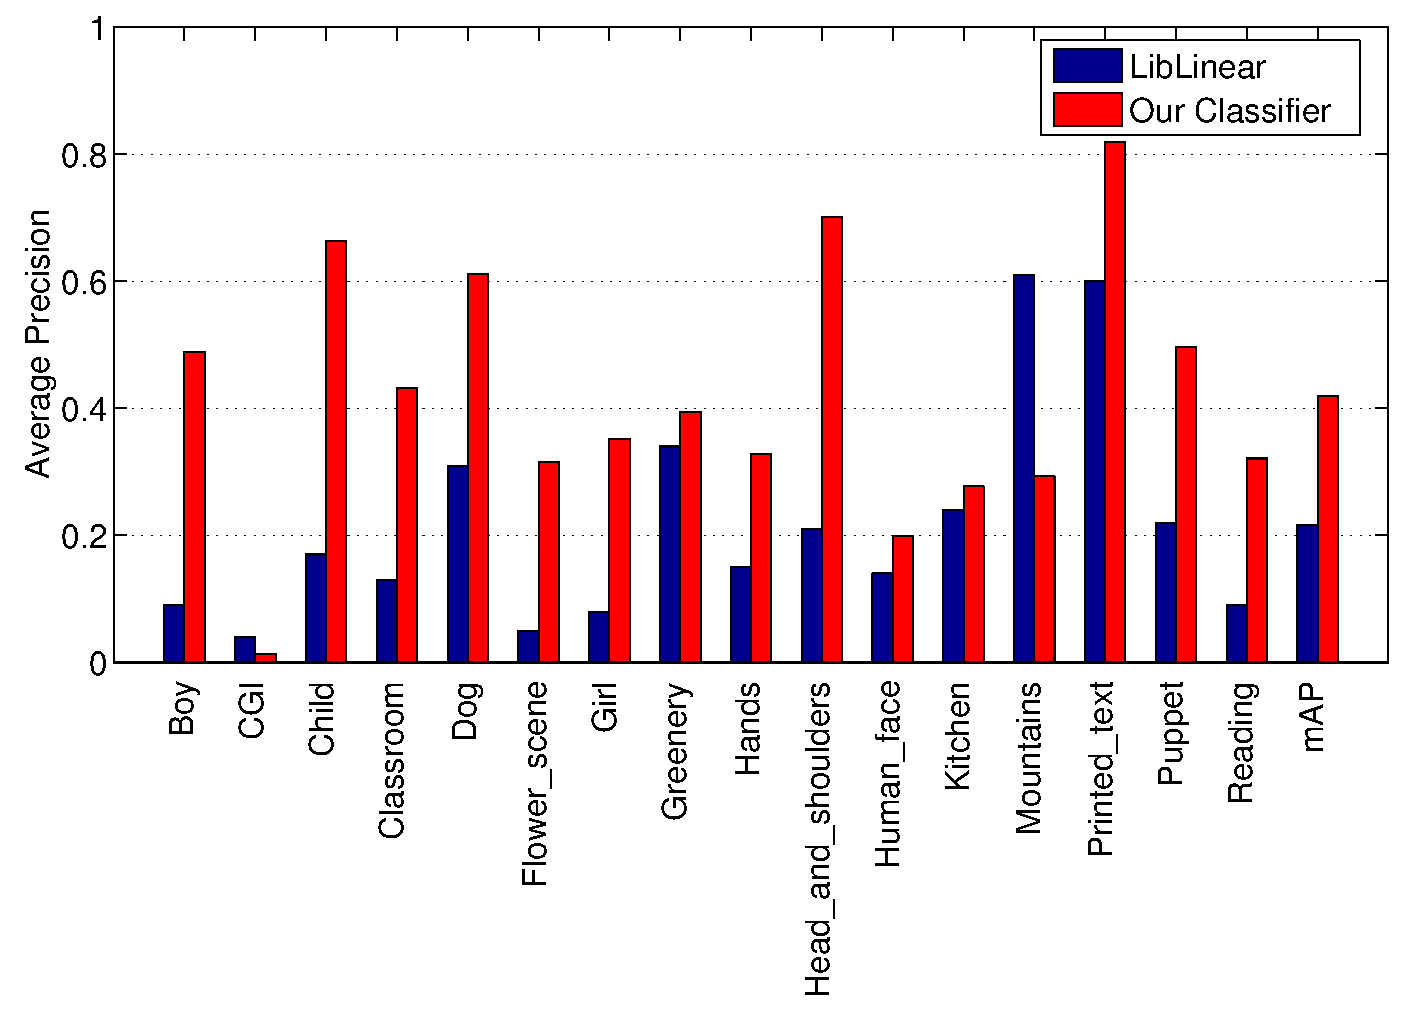
\includegraphics[width=0.48\textwidth]{fig6.pdf}
\centering
\caption{Detailed performance comparison between Liblinear classifier and educational ensemble classifier.} \label{fig:fig6}
\end{figure}


% Table generated by Excel2LaTeX from sheet 'Sheet1'
%\begin{table*}[htbp]\scriptsize
%  \centering
%  \caption{Number of Web images in training dataset}
%    \begin{tabular}{r|r|r|r|r|r|r|r|r|r|r|r}
%    \hline
%    \hline
%    \textit{CD} & 454   & \textit{Sofa} & 544   & \textit{Banana} & 420   & \textit{Gorilla} & 199   & \textit{Cityscape} & 550   & \textit{Female\_adult} & 3609 \\
%    \textit{TV} & 286   & \textit{Toys} & 1021  & \textit{Beaker} & 209   & \textit{Kitchen} & 564   & \textit{Classroom} & 804   & \textit{Historic\_pic} & 1460 \\
%    \textit{Boy} & 544   & \textit{Tree} & 443   & \textit{Cannon} & 623   & \textit{Leopard} & 385   & \textit{Mountains} & 843   & \textit{Mars\_surface} & 191 \\
%    \textit{CGI} & 438   & \textit{Beach} & 1567  & \textit{Castle} & 1098  & \textit{Library} & 276   & \textit{Night\_sky} & 1422  & \textit{Math\_formula} & 109 \\
%    \textit{Car} & 6449  & \textit{Cards} & 394   & \textit{Charts} & 3578  & \textit{Printer} & 709   & \textit{Satellite} & 340   & \textit{Oil\_painting} & 828 \\
%    \textit{Cat} & 1115  & \textit{Chess} & 1016  & \textit{Drawer} & 961   & \textit{Reading} & 479   & \textit{Xylophone} & 584   & \textit{Paint\_colors} & 480 \\
%    \textit{Cow} & 426   & \textit{Child} & 647   & \textit{Flower} & 825   & \textit{Rooster} & 486   & \textit{Animations} & 444   & \textit{Printed\_text} & 4080 \\
%    \textit{Dog} & 2352  & \textit{Crowd} & 1240  & \textit{Galaxy} & 297   & \textit{Volcano} & 540   & \textit{Auditorium} & 648   & \textit{Audience\_view} & 239 \\
%    \textit{Eye} & 215   & \textit{Glass} & 655   & \textit{Insect} & 3242  & \textit{Writing} & 216   & \textit{Bike\_wheel} & 552   & \textit{Block\_diagram} & 587 \\
%    \textit{Fox} & 203   & \textit{Globe} & 365   & \textit{Monkey} & 1259  & \textit{Airplane} & 3383  & \textit{Calculator} & 295   & \textit{Computer\_room} & 482 \\
%    \textit{Map} & 765   & \textit{Hands} & 1200  & \textit{Office} & 154   & \textit{Bathroom} & 951   & \textit{Caricature} & 911   & \textit{Factory\_inside} & 543 \\
%    \textit{Sky} & 3428  & \textit{Hippo} & 161   & \textit{Parade} & 1054  & \textit{Building} & 1029  & \textit{Cereal\_box} & 661   & \textit{Produced\_video} & 264 \\
%    \textit{Baby} & 1394  & \textit{Horse} & 2025  & \textit{Pigeon} & 790   & \textit{Corridor} & 332   & \textit{Laboratory} & 731   & \textit{Tennis\_racquet} & 382 \\
%    \textit{Ball} & 345   & \textit{Lemon} & 740   & \textit{Planet} & 201   & \textit{Elephant} & 347   & \textit{Light\_bulb} & 781   & \textit{Computer\_screen} & 839 \\
%    \textit{Bear} & 352   & \textit{Mouse} & 890   & \textit{Puppet} & 217   & \textit{Greenery} & 1068  & \textit{Male\_adult} & 2933  & \textit{President\_nixon} & 172 \\
%    \textit{Bird} & 885   & \textit{Pills} & 398   & \textit{Rabbit} & 331   & \textit{Keyboard} & 949   & \textit{Mars\_rover} & 153   & \textit{President\_obama} & 433 \\
%    \textit{Book} & 309   & \textit{Pizza} & 1162  & \textit{Racoon} & 250   & \textit{Monument} & 4366  & \textit{Playground} & 896   & \textit{Chemical\_formula} & 374 \\
%    \textit{Desk} & 850   & \textit{Plant} & 707   & \textit{Rocket} & 623   & \textit{Portrait} & 14747 & \textit{Presenting} & 1291  & \textit{Light\_microscopy} & 470 \\
%    \textit{Face} & 4906  & \textit{Rhino} & 215   & \textit{Soccer} & 834   & \textit{Pyramids} & 316   & \textit{Snow\_scene} & 2388  & \textit{President\_carter} & 233 \\
%    \textit{Fish} & 574   & \textit{River} & 490   & \textit{Spider} & 205   & \textit{Sandwich} & 1018  & \textit{Sunglasses} & 670   & \textit{President\_reagan} & 148 \\
%    \textit{Foot} & 286   & \textit{Scale} & 427   & \textit{Statue} & 914   & \textit{Soldiers} & 898   & \textit{Two\_people} & 3767  & \textit{Washer\_and\_dryer} & 1114 \\
%    \textit{Frog} & 280   & \textit{Sheep} & 195   & \textit{Berries} & 361   & \textit{Speakers} & 352   & \textit{Underwater} & 1210  & \textit{Weather\_forecast} & 357 \\
%    \textit{Girl} & 710   & \textit{Skull} & 293   & \textit{Bicycle} & 1196  & \textit{Ambulance} & 1026  & \textit{Watermelon} & 734   & \textit{American\_football} & 589 \\
%    \textit{Lion} & 239   & \textit{Snake} & 535   & \textit{Cartoon} & 289   & \textit{Astronaut} & 300   & \textit{Power\_plant} & 254   & \textit{President\_gw\_bush} & 303 \\
%    \textit{Moon} & 289   & \textit{Stove} & 931   & \textit{Cockpit} & 694   & \textit{Bar\_chart} & 347   & \textit{Sport\_field} & 2630  & \textit{Grocery\_store\_shelf} & 372 \\
%    \textit{Road} & 455   & \textit{Tiger} & 395   & \textit{Drawing} & 360   & \textit{CD\_player} & 147   & \textit{Water\_scene} & 1897  & \textit{President\_washington} & 116 \\
%    \textit{Sink} & 188   & \textit{X\_ray} & 523   & \textit{Giraffe} & 362   & \textit{Cellphone} & 731   & \textit{Wheat\_field} & 405   & \textit{Periodic\_table\_of\_elements} & 228 \\
%    \hline
%    \hline
%    \end{tabular}%
%  \label{tbl:large}%
%\end{table*}%

\begin{figure}[h]
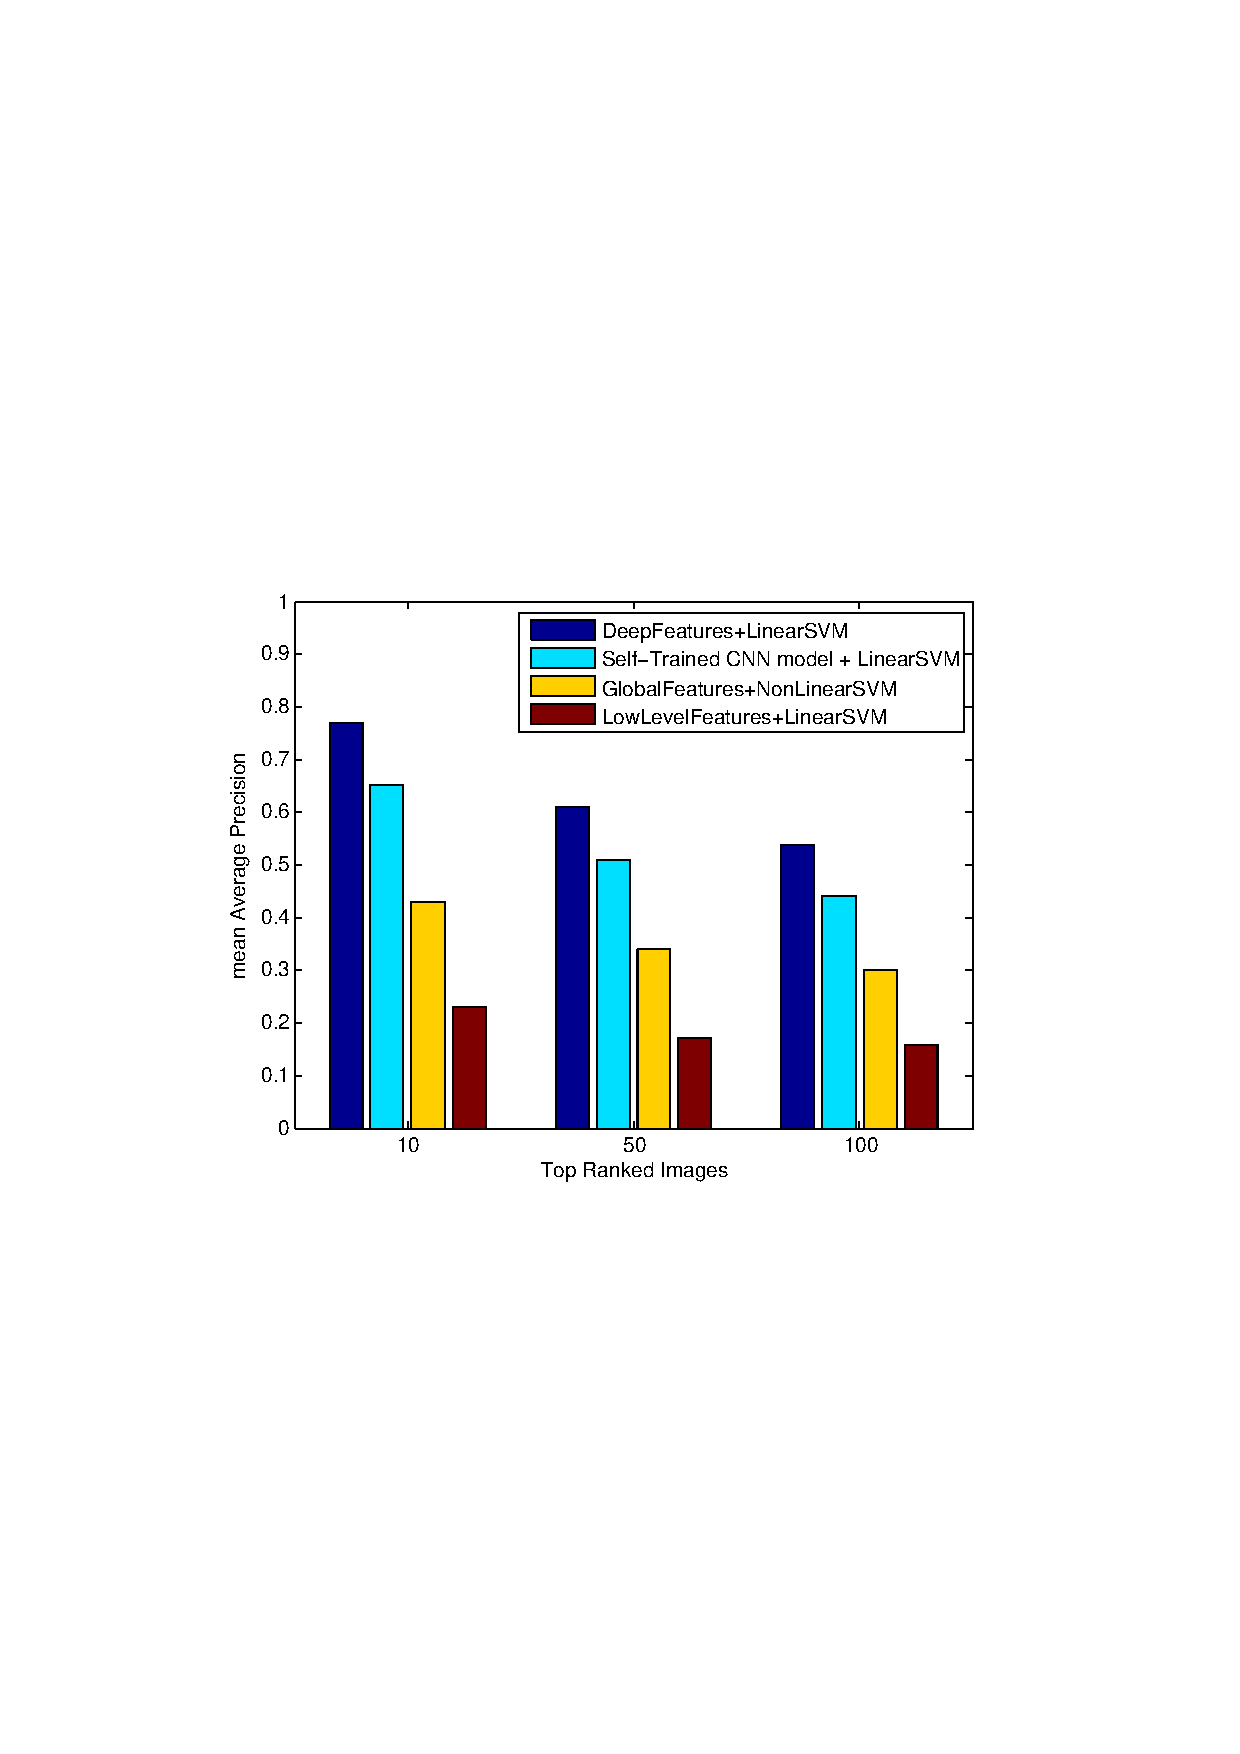
\includegraphics[width=0.48\textwidth]{fig8.pdf}
\centering
\caption{Performance comparison in mean Average Precision~(mAP) with low-level features, global features and deep features.} \label{fig:fig6}
\end{figure}


\begin{figure*}[h]
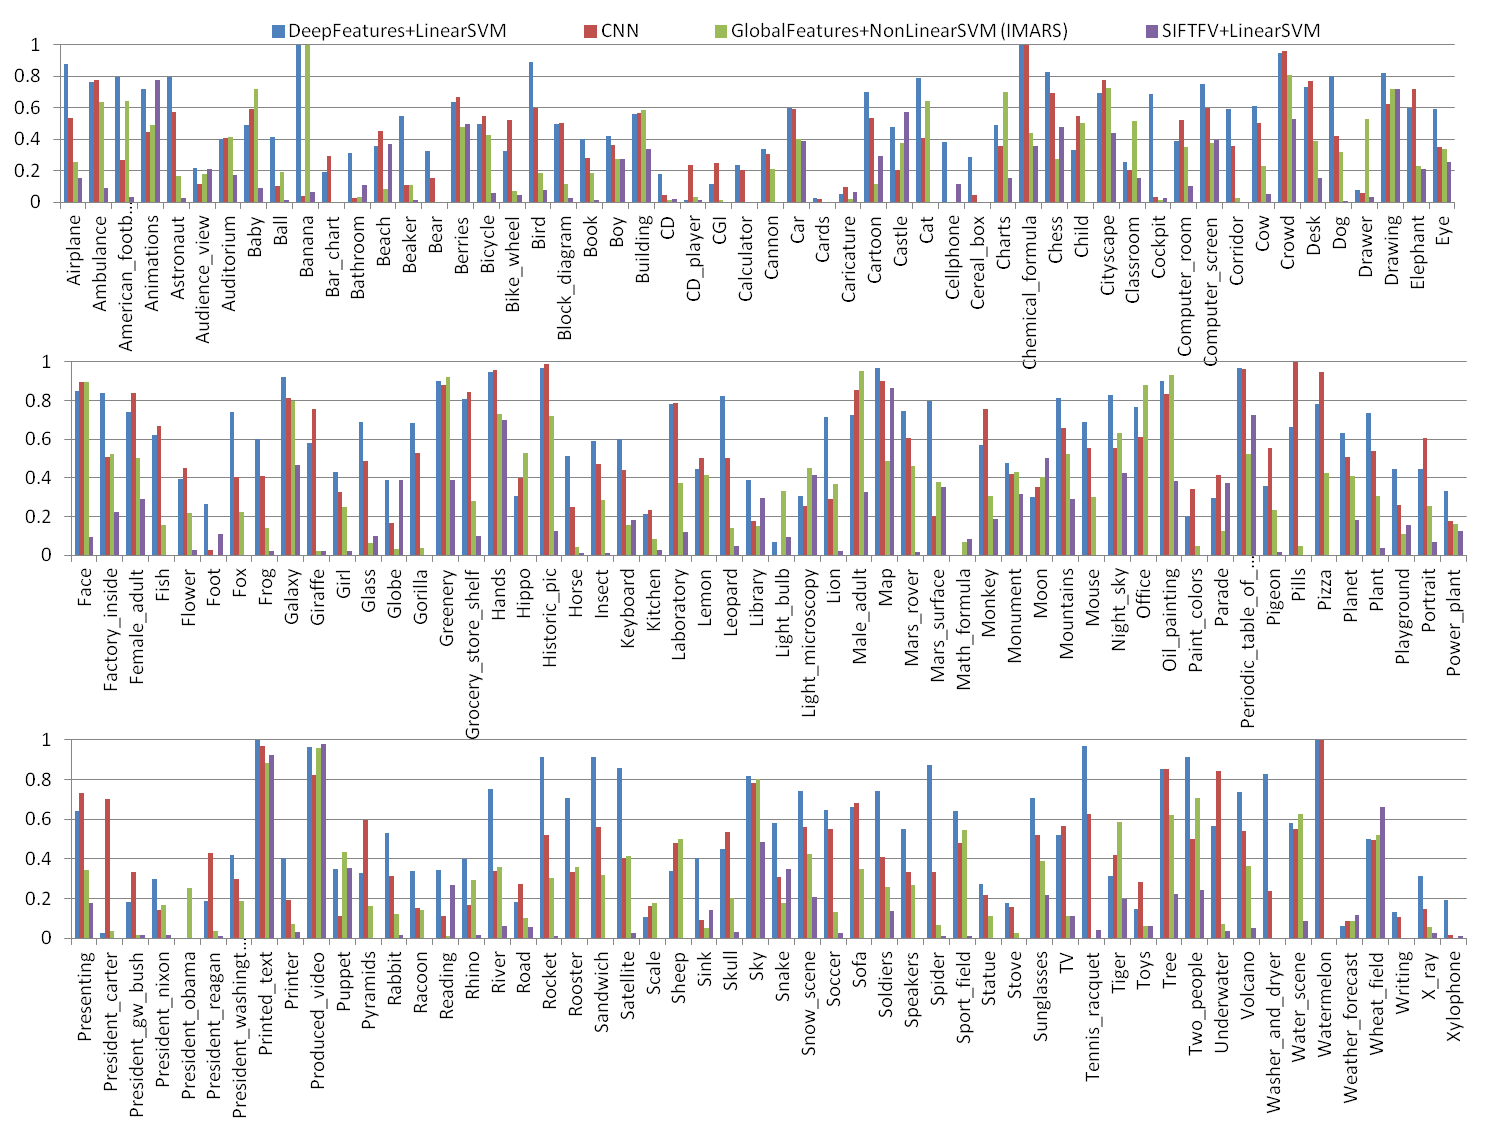
\includegraphics[width=\textwidth]{fig9.png}
\centering
\caption{Detailed experimental comparison of 162 categories Average Precision~(mAP) with low-level features, global features and deep features.} \label{fig:fig6}
\end{figure*}

\begin{figure}[h]
\centering
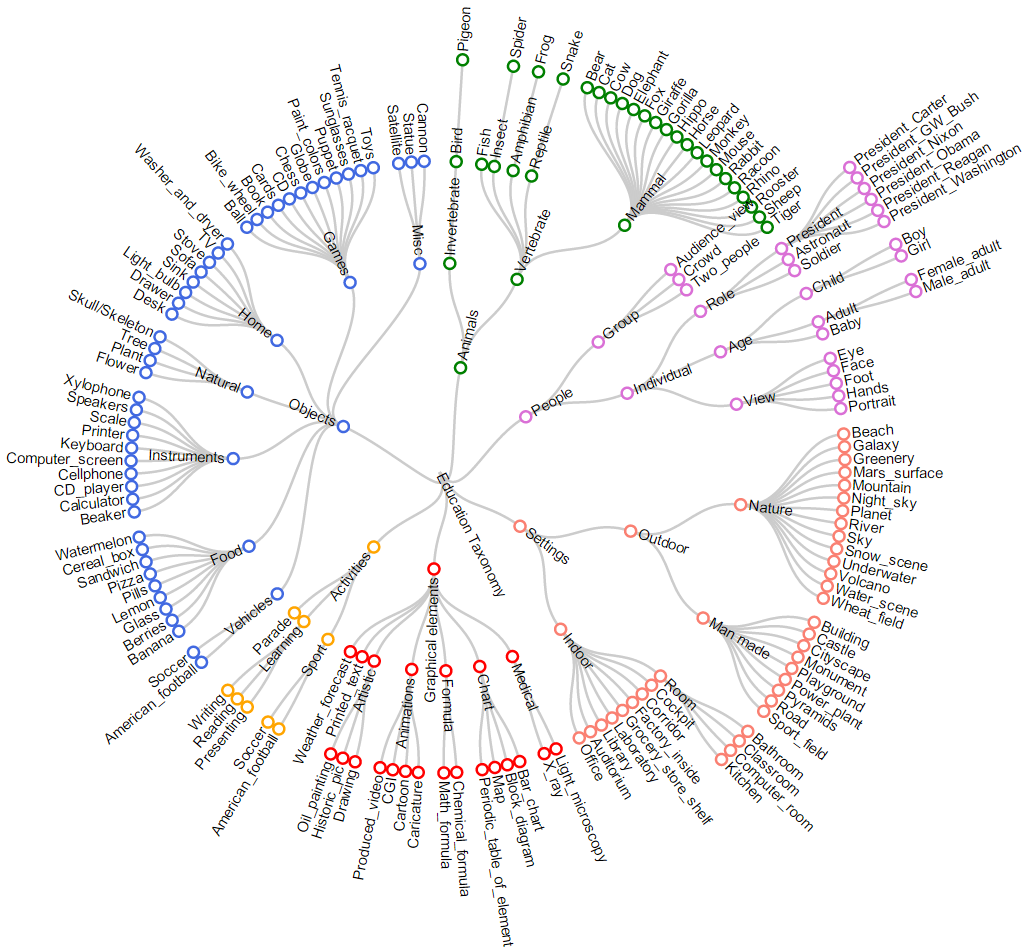
\includegraphics[width=0.5\textwidth]{fig10.png}
\caption{Visualization of hierarchical taxonomy tree for 162 categories in the training dataset.} \label{fig:fig6}
\end{figure}

\begin{figure}[h]
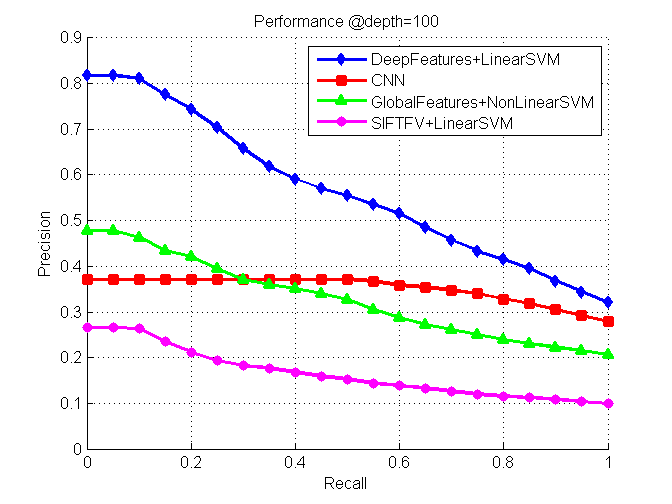
\includegraphics[width=0.5\textwidth]{fig11.png}
\centering
\caption{Performance comparison in precision and recall at top 100 ranked images.} \label{fig:fig6}
\end{figure}

\begin{figure}[h]
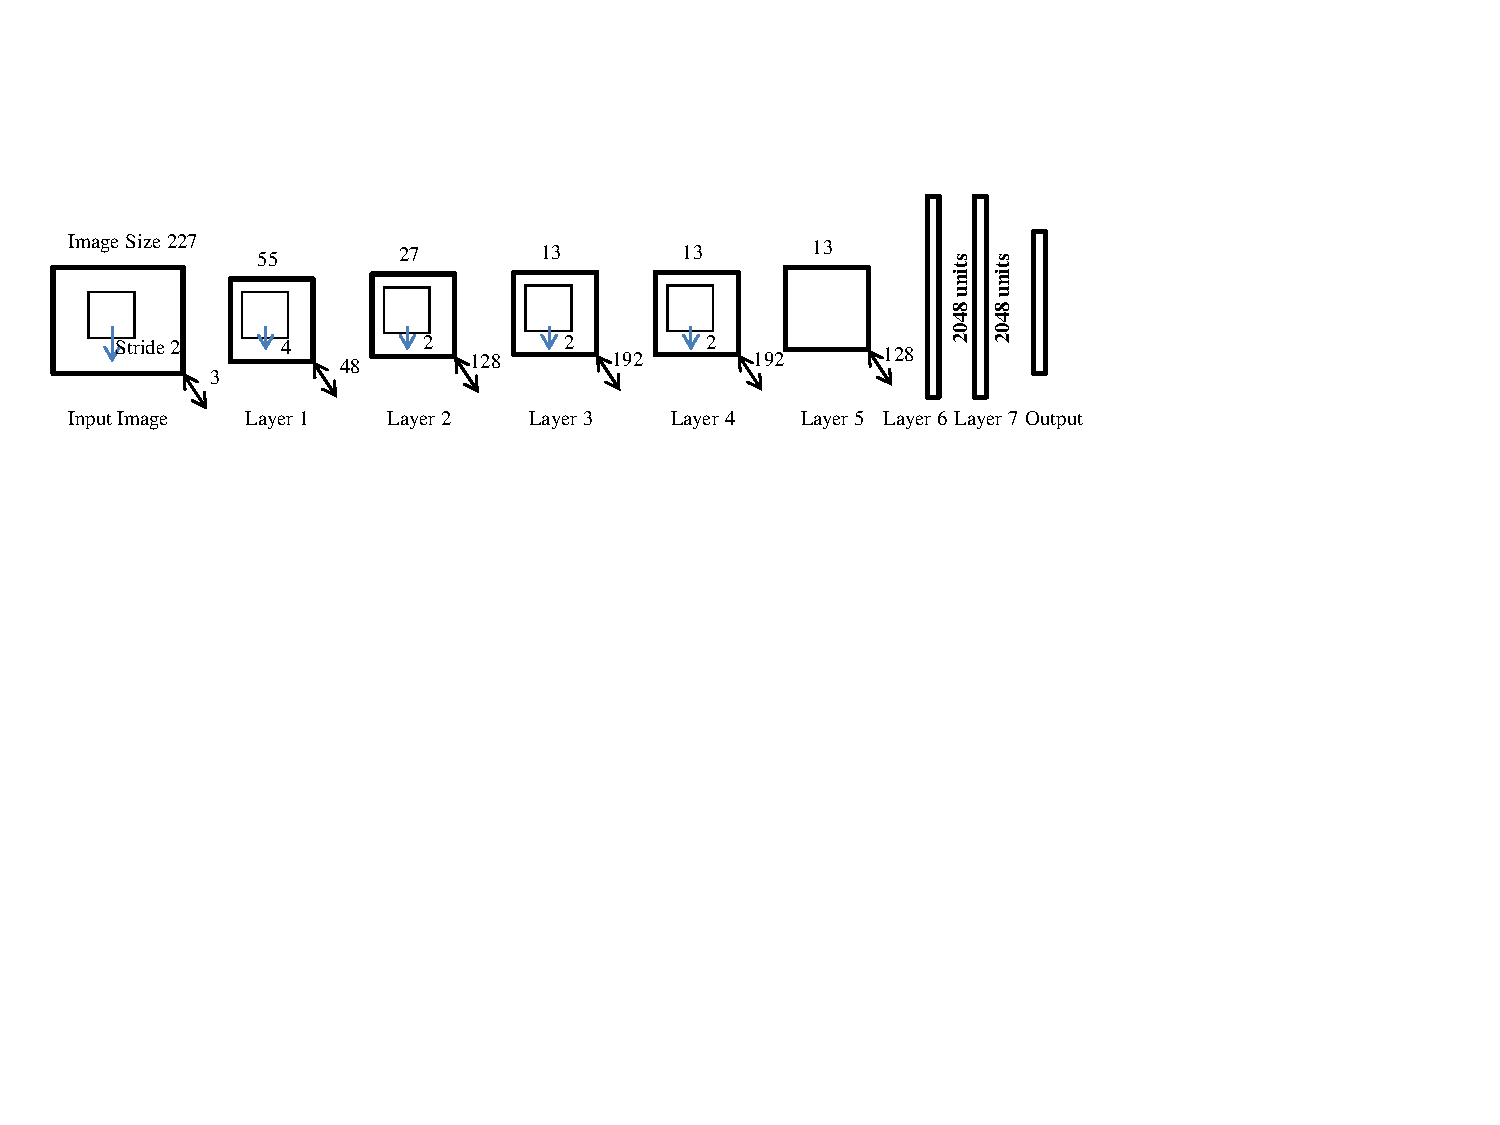
\includegraphics[width=0.5\textwidth]{fig12.pdf}
\centering
\caption{Architecture of our CNN network. We take a 227 $\times$ 227 $\times$ 3 image as the input and convolve it with 48 different first layer filters, each of which with the size 7 $\times$
7, using a stride of two in both dimensions.} \label{fig:fig6}
\end{figure}

\bibliographystyle{abbrv} \scriptsize
\begin{thebibliography}{1}

%\bibitem{Lee_10}
%H. Chang, H. Kim, S. Li, J. Lee and D. Lee.
%\newblock Comparative study on subject classification academic videos using noisy transcripts.
%\newblock In {\em ICSC}, 2010.

\bibitem{TRECVID07}
M.~Campbell, A. Haubold, M. Liu, A. Natsev and J. R. Smith.
\newblock IBM research TRECVID-2007 video retrieval system.
\newblock In {\em NIST TRECVID Workshop}, 2007.


\bibitem{Michele_TMM13}
M. Merler, B. Huang, L. Xie, G. Hua and A. Natsev.
\newblock Semantic model vectors for complex video event recognition.
\newblock In {\em IEEE Transaction on Multimedia}, vol. 14, no. 1, pp. 88-101, 2012.

\bibitem{CAFFE}
Y. Jia.
\newblock {Caffe}: An Open Source Convolutional Architecture for Fast Feature Embedding.
\newblock {\em \url{http://caffe.berkeleyvision.org/}}, 2013.

\bibitem{survey}
I. Allen and J. Seaman.
\newblock Changing course: ten years of tracking online education in the united states.
\newblock In {\em Annual Report of Babson Survey Research Group}, 2013.

\bibitem{IMARS}
R. Yan, T. Tesic and J. R. Smith.
\newblock Model-shared subspace boosting for multi-label classification.
\newblock In {\em ACM SIGKDD Conference on Knowledge Discovery and Data Mining},~2007.


\bibitem{ICME03}
J. Smith, M. Naphade and A. Natsev.
\newblock Multimedia semantic indexing using model vectors.
\newblock In {\em Proceedings of the IEEE Conference on Multimedia and Expo}, 2003.


\bibitem{Karpathy_CVPR14}
A. Karpathy, G. Toderici, S. Shetty, T. Leung, R. Sukthankar and L. Fei-Fei.
\newblock Large-scale video classification with convolutional neural networks.
\newblock In {\em Proceedings of the IEEE conference on Computer Vision and Pattern Recognition}, 2014.


\bibitem{Fergus_ECCV14}
M. Zeiler and R. Fergus.
\newblock Visualizing and understanding convenlutional networks.
\newblock In {\em Proceedings of the IEEE European Conference on Computer Vision}, 2014.


\bibitem{Alex_NIPS12}
A. Krizhevsky, I. Sutskever and G.E. Hinton.
\newblock ImageNet classification with deep convolutional neural networks.
\newblock In {\em Proceedings of Advanced in Neural Inforamtion Processing System}, 2012.


\bibitem{Caltech256}
G. Griffin, A. Holub and P. Perona.
\newblock The caltech 256.
\newblock In {\em Caltech Technical Report}, 2006.

\bibitem{Liblinear}
R. Fan, K. Chang, C. Hsieh, X. Wang and C. Lin.
\newblock LIBLINEAR: a library for large linear classification.
\newblock In {\em Journal of Machine Learning Research}, vol. 9, no. 4, pp. 1871-1874, 2008.

\bibitem{ICME06}
S. Ebadollahi, L. Xie, S. Chang and J. Smith.
\newblock Visual event detection using multi-dimesional concept dynamics.
\newblock In {\em Proceedings of the ACM International Conference on Multimedia and Expo}, 2006.

\bibitem{KDD04}
A. Natsev, M. Naphade and J. Smith.
\newblock Semantic representation, search and mining of multimedia content.
\newblock In {\em ACM SIGKDD Conference on Knowledge Discovery and Data Mining}, 2004.

\bibitem{Early_Fusion}
X. Peng, L. Wang, X. Wang and Y. Qiao.
\newblock Bag of Visual Words and Fusion Methods for Action Recognition: Comprehensive Study and Good Practice.
\newblock In {\em arXiv}, 2014.


\bibitem{CNN_off_the_shelf}
A. Razavian, H. Azizpour, J. Sullivan and S. Carlsson.
\newblock CNN Features off-the-shelf: an astounding Baseline for recognition.
\newblock In {\em arXiv}, 2014.

\bibitem{CVPR14}
K. Simonyan and A. Zisserman.
\newblock Two-stream conventional networks for action recognition in videos.
\newblock In {\em Proceedings of the IEEE conference on Computer Vision and Pattern Recognition}, 2014.

\bibitem{Boostroost}
X. Li, C. Snoek, M. Worring, D. Koelma and A. Smeulders.
\newblock Boostrapping visual categorization with relevant negatives.
\newblock In {\em IEEE Transaction on Multimedia}, vol. 15, no. 4, pp. 933 - 945, 2013.

\bibitem{LSVRC}
Large scale visual recogntion challenge.
\newblock {\em \url{http://www.image-net.org/challenges/LSVRC/2012/}}, 2012.

\bibitem{SpeechRecogntion}
G. Hinton, L. Deng, D. Yu, G. Dahl, A. Mohamed and N. Jaitly.
\newblock Deep neural networks for acoustic modeling in speech recognition:
The shared views of four research groups.
\newblock In {\em IEEE Signal Processing Magazine}, vol. 29, no. 6, pp. 82-97, 2008.

\bibitem{YLecun}
Y. Lecun, K. Kavukcuoglu and C. Farabet.
\newblock Convolutional networks and applications in vision.
\newblock In {\em Proceedings of the IEEE International Symposium on Circuits and Systems}, 2010.


\bibitem{ImageNet_challenge}
O. Russakovsky, J. Deng, H. Su and A. Berg.
\newblock ImageNet large scale visual recogntion challenge.
\newblock In {\em arXiv}, 2014.


\bibitem{Attila}
H. Soltau, G. Saon, and B. Kingsbury.
\newblock The IBM Attila speech recognition toolkit.
\newblock In {\em Proceedings of the IEEE Spoken Language Technology Workshop}, 2010.


\bibitem{Kaldi}
D. Povey et al.
\newblock Deep Neural Networks in Kaldi.
\newblock {\em \url{http://kaldi.sourceforge.net/dnn.html}}, 2013.

\bibitem{OverFeat}
P. Sermanet, D. Eigen, X. Zhang, M. Mathieu, R. Fergus, Y. LeCun.
\newblock OverFeat: Integrated Recognition, Localization and Detection using Convolutional Networks.
\newblock In {\em arXiv}, 2014.


\bibitem{Theano}
J. Bergstra, O. Breuleux, F. Bastien, P. Lamblin, R. Pascanu, G. Desjardins, J. Turian, D. Warde-Farley and Y. Bengio.
\newblock Theano: A CPU and GPU Math Expression Compiler.
\newblock In {\em Proceedings of the Python for Scientific Computing Conference}, 2010.


\bibitem{Classemes}
A. Bergamo and  L.Torresani.
\newblock Classemes and Other Classifier-based Features for Efficient Object Categorization.
\newblock {\em IEEE Transaction on Pattern Analysis and Machine Intelligence}, vol.36, no.10, pp.1988 - 2001, 2014.


\bibitem{VastMM}
A. Haubold and J. Kender.
\newblock VAST MM: Multimedia Browser for Presentation Video.
\newblock In {\em Proceedings of the ACM International Conference on Image and video retrieval}, 2007.

\bibitem{talkminer}
J. Adcock, M. Cooper, L. Denoue, H. Pirsiavash and L. Rowe.
\newblock TalkMiner: A lecture webcast search engine.
\newblock In {\em Proceedings of the ACM Conference on Multimedia}, 2010.

\bibitem{MED}
L. Cao et al.
\newblock IBM Research TRECVID-2012 Multimedia Event Detection (MED) Systems.
\newblock In {\em Techical Report}, 2012.

\bibitem{Laptev_CVPR08}
I. Laptev, M. Marszalek, C. Schmid and B. Rozenfeld.
\newblock Learning realistic human actions from movies.
\newblock In {\em Proceedings of the IEEE Conference on Computer Vision and Pattern Recognition}, 2008.


\bibitem{HOG}
N. Dalal and B. Triggs.
\newblock Histogram of oriented gradients for human detection.
\newblock In {\em Proceedings of the IEEE Conference on Computer Vision and Pattern Recognition}, 2005.


\bibitem{HOF}
N. Dalal and B. Triggs.
\newblock Human detection using oriented histograms of flow and appearance.
\newblock In {\em Proceedings of the IEEE European Conference on Computer Vision}, 2006.


\bibitem{WangHeng_BMVC09}
H. Wang, M.~M.~Ullah, A.~Klaser, I.~Laptev and C. Schmid.
\newblock Evaluation of local spatio-temporal features for action recognition.
\newblock In {\em Proceedings of the IEEE British Machine Vision Conference}, 2009.


\bibitem{WangHeng_CVPR11}
H. Wang, A.~Klaser, C. Schmid and C.~L.~Liu.
\newblock Action recognition by dense trajectories.
\newblock In {\em Proceedings of the IEEE European Conference on Computer Vision}, 2011.

\bibitem{WangHeng_ICCV13}
H. Wang and C. Schmid.
\newblock Action recognition with improved trajectories.
\newblock In {\em Proceedings of the IEEE International Conference on Computer Vision}, 2013.


\bibitem{Jegou13}
M. Jain, H.~Jegou, and P. Bouthemy.
\newblock Better exploiting motion for better action recogntion.
\newblock In {\em Proceedings of the IEEE Conference on Computer Vision and Pattern Recognition}, 2013.


\bibitem{fishervector}
F.~Perronnin, J. Sanchez and T. Mensink.
\newblock Improving the Fisher kernel for large-scale image classification.
\newblock In {\em Proceedings of the IEEE European Conference on Computer Vision}, 2010.


\bibitem{huang07}
H.~Jhuang, T.~Serre, L.~Wolf and T.~Poggio.
\newblock A biologically inspired system for action recognition.
\newblock In {\em Proceedings of the IEEE International Conference on Computer Vision}, 2007.


\bibitem{HMDB}
H.Kuehne, H.~Jhuang, T.~Poggio and T.~Serre.
\newblock HMDB: A large video database for human motion recogntion.
\newblock In {\em Proceedings of the IEEE International Conference on Computer Vision}, 2011.

\bibitem{Fergus10}
G.~W. Tayleor, R.~Fergus, Y.~LeCun and C.~Bregler.
\newblock Conveolutional learning of spatio-temporla features.
\newblock In {\em Proceedings of the IEEE European Conference on Computer Vision}, 2010.

\bibitem{Kaiyu13}
S. Ji, W. Xu, M. Yang, and K. Yu.
\newblock 3D convolutional neural networks for human action recognition.
\newblock {\em IEEE Transaction on Pattern Analysis and Machine Intelligence}, vol.35, no.1, pp.221 - 231, 2013.

\bibitem{VLFeat}
A. Vedaldi and B. Fulkeson.
\newblock VLFeat: An open and portable library of computer vision algorithms. 2008.

\end{thebibliography}

\end{document}
